\ifx\mainfile\undefined
%  ========================================================================
%  Copyright (c) 2006-2011 The University of Washington
%
%  Licensed under the Apache License, Version 2.0 (the "License");
%  you may not use this file except in compliance with the License.
%  You may obtain a copy of the License at
%
%      http://www.apache.org/licenses/LICENSE-2.0
%
%  Unless required by applicable law or agreed to in writing, software
%  distributed under the License is distributed on an "AS IS" BASIS,
%  WITHOUT WARRANTIES OR CONDITIONS OF ANY KIND, either express or implied.
%  See the License for the specific language governing permissions and
%  limitations under the License.
%  ========================================================================
%
 
\documentclass [11pt, twoside] {uwthesis}

\usepackage{color}
\usepackage{url}
\usepackage{amsmath}
\usepackage{amsfonts}
\usepackage[bookmarks,
	hidelinks,
	plainpages=false,
	pdfpagelabels,
	pagebackref=true,
            ]{hyperref}
\renewcommand*{\backref}[1]{}% for backref < 1.33 necessary
\renewcommand*{\backrefalt}[4]{%
  \ifcase #1 %
    (No citations.)%
  \or
    (Cited on page #2.)%
  \else
    (Cited on pages #2.)%
  \fi
}

\newcommand{\biburl}[1]{{\tt<}\url{#1}{\tt>}}

\hypersetup{%
pdfauthor = {Daniel Chaim Halperin},
pdftitle = {Simplifying the Configuration of 802.11 Wireless Networks with Effective SNR},
pdfsubject = {Ph.D. Dissertation},
pdfkeywords = {},
pdfcreator = {University of Washington, Computer Science and Engineering},
pdfproducer = {},
bookmarksopen = {true},
pdfpagelayout = {TwoColumnRight},
}

\usepackage{footnotebackref}
%%%%%%%%%%%%%%%%%%%%%%%%%%%%%%%%%%%%%%%%%%%%%%%%%%%%%%
%%%        Formatting sections                     %%%
%%%%%%%%%%%%%%%%%%%%%%%%%%%%%%%%%%%%%%%%%%%%%%%%%%%%%%
\newcommand{\algref}[1]{Algorithm~\ref{#1}}
\newcommand{\chapref}[1]{Chapter~\ref{#1}}
\renewcommand{\eqref}[1]{Equation~\ref{#1}}
\newcommand{\figref}[1]{Figure~\ref{#1}}
\newcommand{\secref}[1]{\S\ref{#1}}
\newcommand{\tabref}[1]{Table~\ref{#1}}
\newcommand{\heading}[1]{\vspace{4pt}\noindent\textbf{#1}}
\newcommand{\topheading}[1]{\noindent\textbf{#1}}
\newcommand{\noheading}[0]{\vspace{4pt}\noindent}

%%%%%%%%%%%%%%%%%%%%%%%%%%%%%%%%%%%%%%%%%%%%%%%%%%%%%%
%%%        XXX and other warnings                  %%%
%%%%%%%%%%%%%%%%%%%%%%%%%%%%%%%%%%%%%%%%%%%%%%%%%%%%%%
\newcommand{\xxx}[1]{\textit{\color{red}XXX #1}}

%%%%%%%%%%%%%%%%%%%%%%%%%%%%%%%%%%%%%%%%%%%%%%%%%%%%%%
%%%        Units                                   %%%
%%%%%%%%%%%%%%%%%%%%%%%%%%%%%%%%%%%%%%%%%%%%%%%%%%%%%%
\usepackage{xspace}
\newcommand{\unitsep}{\texorpdfstring{\,}{ }}
\def\unit#1{% from: http://www.tex.ac.uk/cgi-bin/texfaq2html?label=csname "Defining a macro from an argument"
  \expandafter\def\csname #1\endcsname{\unitsep\text{#1}\xspace}%
}
\def\varunit#1#2{% from: http://www.tex.ac.uk/cgi-bin/texfaq2html?label=csname "Defining a macro from an argument"
  \expandafter\def\csname #1\endcsname{\unitsep\text{#2}\xspace}%
}
\unit{GHz}
\unit{MHz}
\unit{kHz}
\unit{Gbps}
\unit{Mbps}
\unit{KB}
\unit{dB}
\unit{dBi}
\unit{dBm}
\unit{W}
\unit{mW}
\varunit{uW}{$\mu$W}
\unit{ms}
\varunit{us}{$\mu$s}
\unit{h}
\unit{m}
\unit{s}
\unit{km}
\unit{cm}
\unit{mm}
\varunit{mmsq}{mm$^\text{2}$}
\varunit{insq}{in$^\text{2}$}
\newcommand{\degree}{\ensuremath{^\circ}\xspace}
\newcommand{\degrees}{\degree}
%%%%%%%%%%%%%%%%%%%%%%%%%%%%%%%%%%%%%%%%%%%%%%%%%%%%%%%%%%%%%%%%%%%%%%%%%%%%%%%%%%%%%%
% Euler for math | Palatino for rm | Helvetica for ss | Courier for tt
%
% From: http://www.tug.org/mactex/fonts/LaTeX_Preamble-Font_Choices.html
%%%%%%%%%%%%%%%%%%%%%%%%%%%%%%%%%%%%%%%%%%%%%%%%%%%%%%%%%%%%%%%%%%%%%%%%%%%%%%%%%%%%%%
\renewcommand{\rmdefault}{ppl} % rm
\usepackage[scaled]{helvet} % ss
\usepackage{courier} % tt
\usepackage{eulervm} % a better implementation of the euler package (not in gwTeX)
\normalfont
\usepackage[T1]{fontenc}
%%%%%%%%%%%%%%%%%%%%%%%%%%%%%%%%%%%%%%%%%%%%%%%%%%%%%%%%%%%%%%%%%%%%%%%%%%%%%%%%%%%%%%

%%%%%%%%%%%%%%%%%%%%%%%%%%%%%%%%%%%%%%%%%%%%%%%%%%%%%%
%%%        Figures                                 %%%
%%%%%%%%%%%%%%%%%%%%%%%%%%%%%%%%%%%%%%%%%%%%%%%%%%%%%%
\usepackage{graphicx}
% Caption package both lets you set the spacing between figure and caption
% and also makes the \figref{} point to the right place.
\usepackage[font=bf,aboveskip=6pt,belowskip=-4mm]{caption}
% Allow subfigures, make them bold
\usepackage[bf,BF,small]{subfigure}
% List of figures
\setcounter{lofdepth}{2}  % Print the chapter and sections to the lot

%%%%%%%%%%%%%%%%%%%%%%%%%%%%%%%%%%%%%%%%%%%%%%%%%%%%%%
%%%        Lists with reduced spacing              %%%
%%%%%%%%%%%%%%%%%%%%%%%%%%%%%%%%%%%%%%%%%%%%%%%%%%%%%%
\usepackage{enumitem}

%%%%%%%%%%%%%%%%%%%%%%%%%%%%%%%%%%%%%%%%%%%%%%%%%%%%%%
%%%        Fancy tables                            %%%
%%%%%%%%%%%%%%%%%%%%%%%%%%%%%%%%%%%%%%%%%%%%%%%%%%%%%%
\usepackage{tabulary}
\usepackage{booktabs}

%%%%%%%%%%%%%%%%%%%%%%%%%%%%%%%%%%%%%%%%%%%%%%%%%%%%%%
%%%        Formatting techniques/tools/etc.        %%%
%%%%%%%%%%%%%%%%%%%%%%%%%%%%%%%%%%%%%%%%%%%%%%%%%%%%%%
\newcommand{\term}[1]{\texttt{#1}}

\begin{document}
 
\textpages
\setcounter{chapter}{0} % Set to n-1!
\fi
%%%%%%%%%%%%%%%%%%%%%%%%%%%%%%%%%%

\cleardoublepage
\chapter{Introduction}
\label{chap:intro}

%Wireless communication forms the dominant consumer-facing networking technology in the world. Billions of people worldwide use cellular phones to provide global voice communication service, and in the past decade smartphones have begun to provide digital access to the Internet for mobile connectivity. These innovations have revolutionized the way people interact with their devices, with each other, and with the world.

%Cellular data networks provide mobile connectivity to the Internet over a long range and at relatively low rates. 
Wireless local area networks are used today to connect devices wirelessly at high rates in locations such as caf\'{e}s, shopping malls, corporate offices, and homes. The dominant technology for these networks is Wi-Fi (IEEE~802.11~\cite{80211}), which emerged in 1997 as a way to connect computers wirelessly to a nearby (within 100\m) Internet ``access point'' at rates up to 2\Mbps.

The past fifteen years have seen Wi-Fi technology improve dramatically. Today's commercial Wi-Fi devices come at low cost, have a small physical footprint, and offer dramatically increased speeds of up to 600\Mbps in IEEE~802.11n~\cite{80211n}. Wi-Fi is no longer limited to traditional computing devices such as laptop and desktop computers, but is also being adopted by consumer electronics such as smartphones, printers, speakers, video cameras, televisions, and DVD players. An ABI Research report~\cite{ABI_Research_2010} forecast that more than half of the 1 billion Wi-Fi chipsets shipped in 2011 would be used in consumer electronics.
%, Wi-Fi today connects devices such as laptops, desktops, tablets, and phones to the Internet at high-speed.
%The latest revision to Wi-Fi, called IEEE~802.11n~\cite{80211n}, enables individual devices to transmit data as fast as 600\Mbps.

Because of its rapid adoption in a diverse set of devices, Wi-Fi is poised at the heart of the next networking revolution: The combining of these diverse consumer devices to build rich applications that leverage each device's unique features. This stands in sharp contrast with today's access point model, in which devices only use wireless connectivity to interact with the Internet at large and hence the access point, which provides the only point of contact with the Internet, is a natural point of centralization. To support this shift away from the access point model, a new protocol called Wi-Fi Direct~\cite{wifi_direct} was standardized in late 2010 that enables Wi-Fi devices to form networks that better match their applications. Wi-Fi Direct has seen great uptake: A second ABI Research study~\cite{ABI_Research_2011}, conducted in late 2011, forecast a 50\% annual growth rate for Wi-Fi Direct support and predicted that there will be 2~billion Wi-Fi Direct-enabled devices by 2016.
%The decades-old ``Internet of Things'' vision is becoming a reality, and researchers have begun building systems such as HomeOS~\cite{Dixon_HomeOS} to design, implement, and program applications that run across the devices in a home.

%The next networking revolution will be for local wireless networks, in the enterprise and especially in the home.
%%, short-range, high-rate local area networks in the
%% enterprise and the
%%home that complement cellular networks.
%, these indoor networks will be used to build rich device-to-device applications in a comparably small area and at much higher rates. Wi-Fi (IEEE 802.11) is the dominant consumer wireless technology, and 
%By both dwarfing the speeds of commercial cellular networks and enabling much denser deployments of many devices that use unlicensed spectrum, Wi-Fi is on the cusp of enabling a new generation of rich device-to-device applications.
%Already, consumer electronics have begun gaining Wi-Fi functionality with dramatic uptake: A 2011 ABI Research report measured a 50\% annual growth rate of devices that support Wi-Fi Direct~\cite{wifi_direct} (a new standard protocol for device-to-device networks) and forecasts that there will be 2~billion Wi-Fi Direct-enabled devices by 2016.
%
%With this shift, the decades-old ``Internet of Things'' vision is becoming a reality, and researchers have begun building systems such as HomeOS~\cite{Dixon_HomeOS} to design, implement, and program applications that run across the devices in a home.
%Now that network-ready consumer devices are available, protocols to connect them have been developed, and systems to control them and help them interoperate are being researched, we have most of the pieces to build the home networks that will support these rich new applications. The last networking component, identified in studies of users who have deployed inchoate versions of home networking systems~\cite{Brush_HomeAutomation}, is a reliable, high-bandwidth wireless network to keep these home devices connected.

%This change is happening fast: An ABI Research report from late 2010 forecast the shipment of 1~billion Wi-Fi (IEEE 802.11~\cite{80211}) chipsets in 2011, with more than half of these chipsets used in consumer electronics, handsets, and other mobile devices. 

Despite these technology, standardization, and adoption trends aligning to enable future rich wireless applications, there is one one major challenge:
%Studies of users who have deployed inchoate versions of home networking systems~\cite{Brush_HomeAutomation} identified a need for a reliable, high-bandwidth wireless network to keep these home devices connected. But
%Realizing a Wi-Fi network's significant potential for speed, capacity, and reliability requires that the network be configured to support the set of devices in the network and the applications that users wish to run. The issue is that
\emph{The underlying Wi-Fi technologies and network architectures have become rather complex, and how to configure and control them has become a significant decision problem that presently lacks a simple, comprehensive solution}.

What does it mean to configure a network? In this thesis, I use the term \emph{configuration} to describe an assignment of values to the physical-layer parameters of one or more wireless devices. This includes the choice of operating frequency, transmit power level, transmit rate, how many and which antennas are used, and more. A configuration problem is the task of configuring all of these parameters for one device, for two devices sending together as a link, or for many devices operating at the same time in a wireless network. Configuration problems can therefore be defined as search problems with the goal of finding a good operating point among the configuration space.

The heart of every configuration algorithm is evaluating the performance of a wireless link in a particular operating point. Consider rate selection, the problem of picking the fastest way to transmit data on a wireless link. In the first version of 802.11, released in 1997, the rate selection task consisted of choosing between two modulations to transmit data. Early algorithms just tried both rates and picked the better one. This worked well through 802.11b and 802.11a/g, because with up to 12 different rates to choose from, ``try-it-and see'' algorithms that probed all options, though not perfect, generally sufficed. But trends in Wi-Fi make this probe-based approach much less effective.

First, the configuration space is growing much larger. One reason is technology trends: Modern 802.11n devices achieve their fast rates by relying on the ability to send with multiple antennas. This adds another dimension to the search space---how many antennas are used---and expands the number of rates into the hundreds. The other reason is usage trends: The device-to-device nature of new networks like Wi-Fi Direct means that coordination within a network is no longer limited a client and its access point. Instead, configuring the network requires extensive coordination between pairs and sets of devices in a network, growing the search space exponentially. Finally, wireless devices are increasingly used in changing environments. For instance, wireless devices are increasingly used while mobile, both while walking indoors and in vehicles. This combination of factors means that algorithms to configure the network need to respond faster to match changing channels, while simultaneously choosing from among more possibilities.

This issue affects all configuration problems, not just rate selection. An example configuration problem for a device-to-device network is choosing a multi-hop path between a source and destination device, possibly using intermediate devices as relays. One step in solving this problem involves assessing the performance achievable on each potential link. This should include taking into account the effect of using different rates, number and sets of antennas, and even the quality of using the best among multiple operating channels for each link. This results in a very large configuration space, which proved impractical for probe-based solutions to search because the search will not converge if the channel conditions change. Instead, past solutions to this subproblem tend to assume away most dimensions of the configuration space---e.g., by assuming homogeneous single-antenna nodes and fixing the entire network to a single bitrate, frequency, and transmit power, so that the system need only probe packet delivery for a single rate. This narrows the space to something feasible to probe, but by eliminating much of the configuration space from consideration likely results in relatively poor performance.

An alternative approach to probing uses measurements of the wireless channel to attempt to predict how well an operating point will work. For instance, 802.11 receivers can measure the total amount of power received from the transmitter. Since using slower rates requires less power than using faster rates, this signal strength measurement might serve as a useful indicator of whether a particular rate works. However, in practice this approach does not provide accurate predictions for Wi-Fi links, for fundamental reasons that I discuss below. Some proposals~\cite{Judd_CHARM} attempt to train a mapping between signal strength and rate, but suffer from the same convergence problems as with probing because this mapping must be updated independently for each configuration point.

To get good performance in future wireless networks, configuration algorithms need to be able to take into account the entire configuration space. Fundamentally, this requires the ability to rapidly assess how well each operating point will work. Using past solutions as evidence indicates that the probe-based algorithms used until now will not scale to handle these future systems. Neither will the approaches based on aggregate signal strength information that must be trained for each operating point. Instead, Wi-Fi systems need a way to predict how well an operating point will work without trying it and without requiring online, per-wireless-link calibration.

%In contrast, an 802.11n device in the same situation today must choose between more than 300 different options! The new Wi-Fi Direct protocol now also includes extensive coordination between pairs and sets of devices in a network, growing this space of choices exponentially. Because of the dramatically larger search space brought about by new 802.11n technologies and new Wi-Fi direct protocols, these legacy probing-based solutions can no longer find a good operating point in a reasonable amount of time. This effect is especially problematic if the network changes dynamically as devices are mobile or people move around in the environment---both of which are possible in the intended Wi-Fi Direct applications.

In this dissertation, I provide a practical, effective solution to this problem. In particular, I develop a comprehensive way to inform these complex decision problems using low-level wireless channel measurements. I devise a simple but powerful model that can predict the performance of every operating point in the entire configuration space, using only a small set of measurements and without online training. Because it only uses one or a few measurements, my model can rapidly update its predictions as the channel changes. My approach enables algorithms that can adjust all parameters and quickly adapt to changing conditions, thus enabling the type of configuration algorithms needed to support rich future wireless networks.
%By using a small set of measurements to extrapolate over a wide configuration space, my approach is considerably more practical than probing everything. By using low-level RF information, my approach is considerably more accurate than approaches that only use high-level signal strength information. Thus my approach represents a great tradeoff between these two extremes, maintaining the flexibility and accuracy of probe-based approaches while achieving the simplicity and low overhead of the latter.
%In this context, I demonstrate the practicality of my techniques  using information available in commercial commodity Wi-Fi hardware.

In the rest of this chapter, I first explain the problem in further detail. I then present my hypothesis and explain my approach to solving this problem. I conclude this chapter by discussing the contributions of my work and the organization of the rest of this thesis.

%%%%%%%%%%%%%%%%%%%%%%%%%%%%%%%%%%
\section{The Problem}
\label{sec:intro_problem}
As stated above, a major challenge for Wi-Fi networks today is finding a good configuration in a changing world. To introduce the problem, I present the main configuration problems in these systems, and briefly explain why today's Wi-Fi solutions are insufficient.

\subsection{Configuring a Single Link}
\label{sec:intro_single_link_problems}
The most basic wireless network is a single link (\figref{fig:wifi_link}), in which a transmitter sends data to one receiver, with no other devices present. In this section, I will show that configuring a wireless link to work well involves choosing the right operating point in a large multi-dimensional space. 

\begin{figure}[tp]
	\centering
	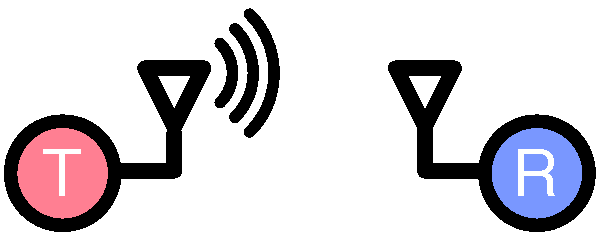
\includegraphics[width=2in]{figures/introduction/single_link_circle.pdf}
	\caption[A single Wi-Fi link]{\label{fig:wifi_link}A single Wi-Fi link, in which the transmitter $T$ sends data to the receiver $R$. No other wireless devices are present.}
\end{figure}

%\subsubsection{Rate Selection}
Perhaps the simplest configuration goal for a wireless link is \define{rate selection}: In most cases, the transmitter should send its data to the receiver using the fastest rate at which it will be successfully received. Sending data more slowly obviously means the transmission takes longer. At the same time, sending faster would be inefficient because the data would not be received, wasting all the airtime and energy consumed during the transmission.

In principle, selecting a rate for a wireless link should be trivial according to the well-known results of communications theory. Whether a transmission sent with a particular modulation and coding scheme is received
%As demonstrated by the seminal works of Ralph Hartley~\cite{Hartley_law} and Claude Shannon~\cite{Shannon_coding,Shannon_capacity}, the maximum data rate that can be delivered over a particular noisy channel (such as a wireless radio link)
is determined entirely by the amount of power delivered to the receiver and the noise level present. This factor is quantified in the \define{signal-to-noise ratio}, or \define{SNR}.
The transmitter need only measure the channel SNR and apply textbook formulas that can compute the error rates of particular modulations. The fastest rate can then be easily selected. This approach is described in \figref{fig:rate_selection_theory}.

\begin{figure}[t]
	\centering
		\subfigure[The theoretical approach to rate selection based on SNR measurement][The theoretical approach to rate selection based on SNR measurement.]{
			\label{fig:rate_selection_theory}
			\hspace{0.1in}
			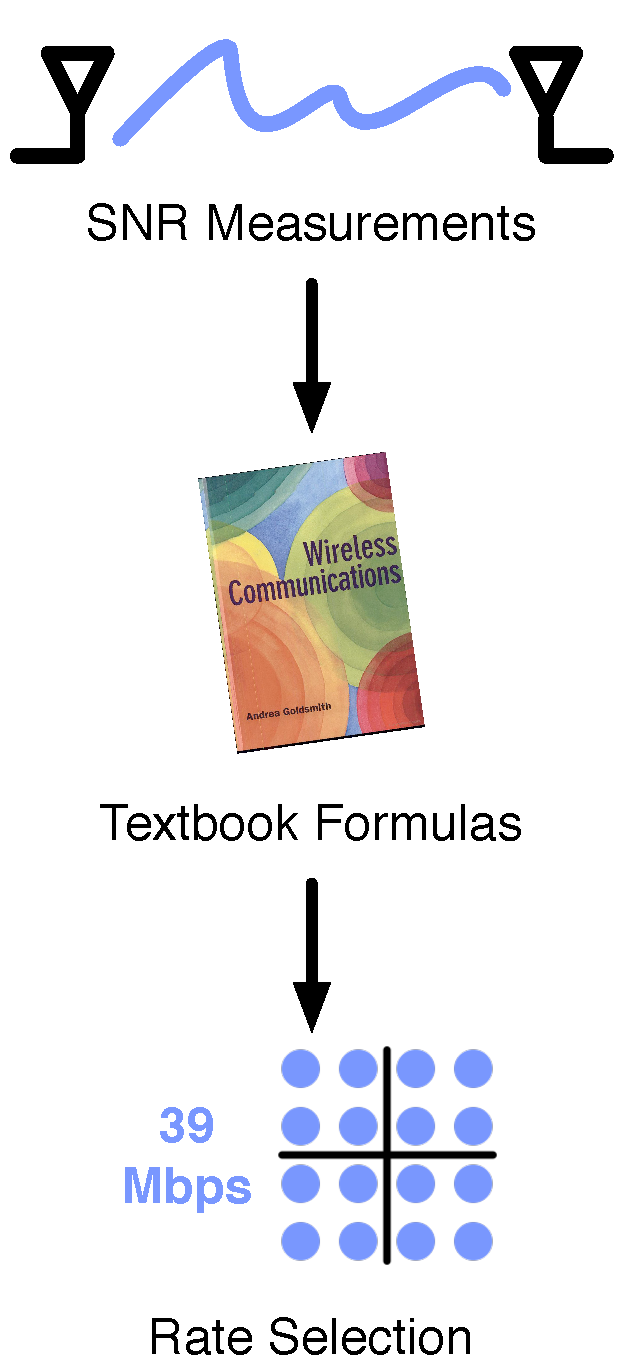
\includegraphics[width=2in]{figures/introduction/rate_selection_theory.pdf}
			\hspace{0.1in}
		}
			\hspace{0.1in}
		\subfigure[The probe-based approach to rate selection][The probe-based approach to rate selection.]{
			\hspace{0.1in}
			\label{fig:rate_selection_practice}
			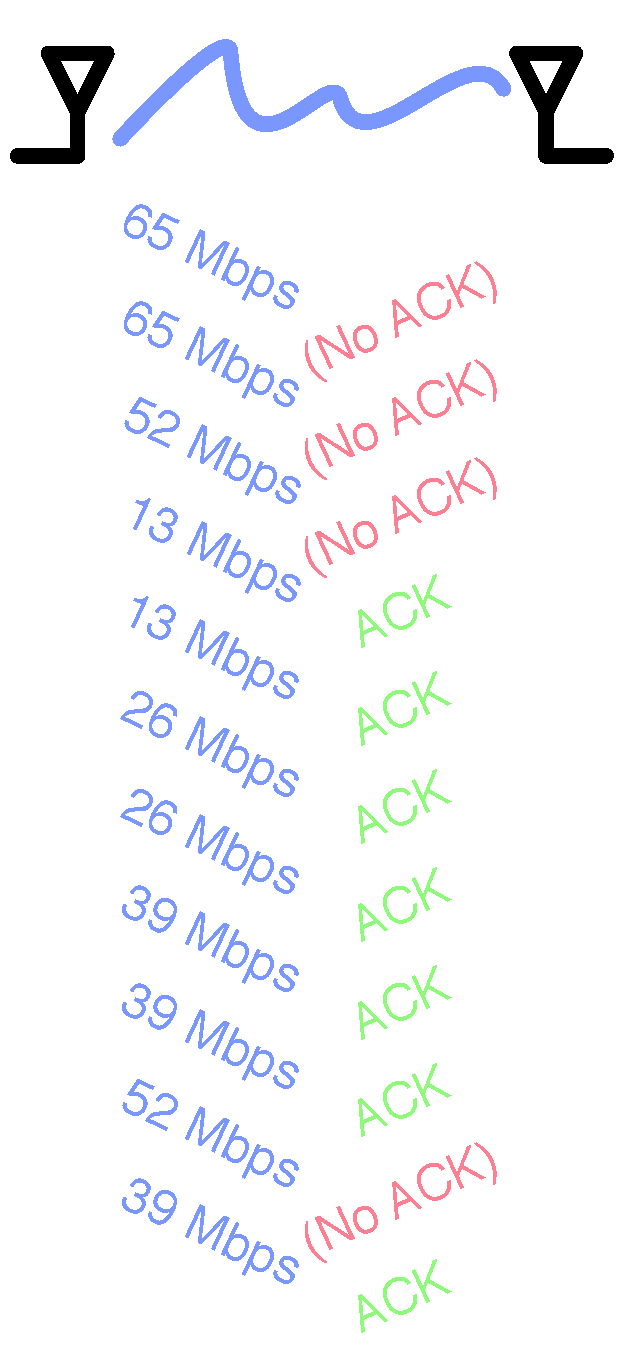
\includegraphics[width=2in]{figures/introduction/rate_selection_practice.pdf}
			\hspace{0.1in}
		}
	\caption[Approaches to rate selection]{\label{fig:rate_selection_algorithms}Approaches to rate selection.}%
\end{figure}

In practice, this approach has never worked for Wi-Fi links. The 802.11 standard defines a channel metric related to the SNR, called the \emph{receive signal strength indicator (RSSI)}, that captures the total amount of power in the channel. In most chipsets, RSSI is indeed a direct measure of the SNR. However, Wi-Fi systems have never used RSSI as more than a coarse indicator of expected performance. There have simply been too many ways in which the observed measurements and actual performance fail to match the predictions of theory. For example, hardware estimates of RSSI can be mis-calibrated, the wireless channel can vary over packet reception, and it can be corrupted by interference~\cite{Camp_rateadapt,Judd_CHARM,Reis_interference}. More fundamentally, the OFDM and MIMO (see \chapref{chap:background}) physical-layer techniques used in 802.11n send independent data on different subchannels with different subchannel SNRs, so that different bits of the packet can have different SNRs. This means that RSSI, which captures only the average SNR of the signal, is fundamentally not a good indicator of performance for Wi-Fi.

Since rate selection based on RSSI has never worked for Wi-Fi, practical systems use \define{rate adaptation} algorithms instead~\cite{Bicket_SampleRate,minstrel,Wong_RRAA}. These algorithms, exemplified by \figref{fig:rate_selection_practice}, are guided search schemes that simply test individual rates to see how well they work. When the loss rate is too high, a lower rate is used; otherwise a higher rate is tested. This approach works well for slowly varying channels and simple links, since the best setting will soon be found.

However, remember the Wi-Fi trends discussed earlier: The transmit configuration of a single Wi-Fi link now includes not just rate, but additional dimensions that take into account the use of multiple antennas or channel widths, and these devices are increasingly being used while mobile. Thus algorithms to configure the rates of these links need to respond more rapidly to match changing conditions, while simultaneously choosing from among more possibilities. As a result, probe-based rate adaptation algorithms are becoming less efficient as these systems become more complex. (I provide results that illustrate this effect in \chapref{chap:rate}.)

Thus far, I have described the challenges inherent to choosing an efficient rate to send data on a wireless link. On its own, this is a hard problem, for which there is a large body of prior work. In addition, I note that rate is only one of many parameters to optimize for a Wi-Fi link. For instance, a transmitter may want to trim excess transmit power to both save energy and reduce interference at nearby receivers. Or a sender might improve a link by selecting a different subset of its transmit antennas, or by applying beamforming techniques to better match the signal to the radio channel. Finally, note that these parameters are not generally independent---changing any one of them can affect the best operating point for another. For instance, switching the operating frequency (of which there are often 10 to 20 options) can dramatically change the RF channel, and this in turn can affect which transmit antennas provide the best link, and how the transmitted signal should be shaped for maximum performance. All of these factors contribute to determining the best way to configure a link. I provide a brief list of link configuration options in \tabref{tab:intro_link_config}.

\begin{table}[tp]
	\centering
	\begin{tabular}{lr}
	\toprule
		Parameter & Number of values \\
	\midrule
		Rate & 8 \\
		Number of spatial streams & 4\\
		Operating channel & $\approx$30 \\
		Channel width & 2 (some proposals use many more)\\
		Transmit power level & $\approx$30 \\
		Transmit antenna set & 6 (for up to 3 streams) \\
		Receive antenna set & 6 (for up to 3 streams) \\
	\bottomrule
	\end{tabular}
	\caption[A list of link configuration parameters]{\label{tab:intro_link_config}A list of link configuration parameters.}
\end{table}


In practice, the solution taken by hardware/driver manufacturers (and by researchers) is to simply ignore most of these dimensions. For instance, only Intel's \program{iwlwifi} driver, out of all the 802.11n drivers in the Linux kernel driver, adapts the transmit antenna set in an online manner. Similarly, few access points and no clients adjust transmit power for ongoing links, instead opting to transmit at the maximum power and guarantee the best link. There are no known research solutions to these problems either. The solutions work well enough for wireless access point networks, mostly due to the simple way in which links are used. Still, these solutions are inefficient for a single link---and in the next section, we will see that the problem gets even more complicated when performing network-level configuration of multiple devices that operate in multiple links.

\subsection{Configuring a Network of Devices}
\label{sec:intro_network_problems}
In this section, I will illustrate how a network of devices has a significantly larger configuration space than a single link. I frame this discussion using the examples in \figref{fig:network_examples}, which represent the three key network-level configuration problems that dense wireless networks like Wi-Fi Direct will have to solve to support device-to-device applications. Depending on the problem being solved, these configuration problems can have increased complexity that is linear in the number of devices (AP selection), quadratic (Multi-hop routing), or even exponential (Spatial reuse).

\begin{figure}[tp]
	\centering
	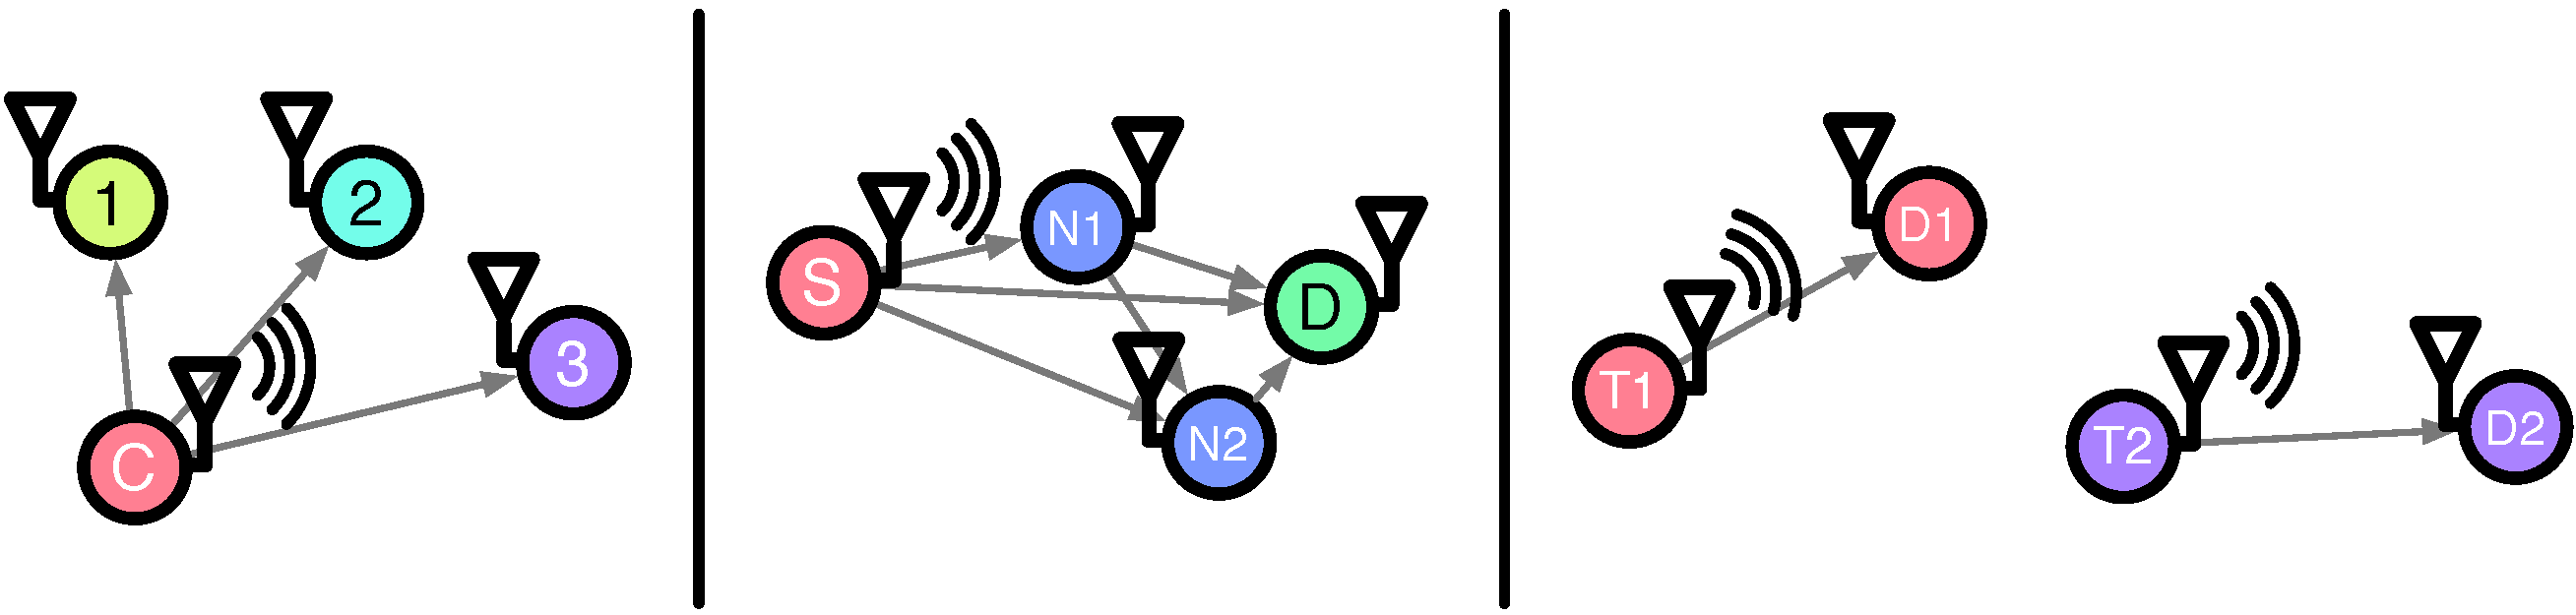
\includegraphics[width=\textwidth]{figures/introduction/network.pdf}
	\caption[The three key configuration problems in multi-device networks]{\label{fig:network_examples} The three key configuration problems in multi-device networks. \textit{Left:} access point selection. \textit{Center:} Multi-hop mesh routing. \textit{Right:} Spatial reuse. }
\end{figure}

\subsubsection{Access Point Selection}
In \figref{fig:network_examples}, on the left, the client $C$ wishes to join the network offered by the access points $AP_1$, $AP_2$, and $AP_3$. The \define{access point selection} problem is simple: The client should connect to the access point that provides the link with the best rate. But in order to choose correctly, the client must accurately evaluate the rate offered by each access point. This in turn means that the client must have a way to assess its rate to each access point, i.e., a solution to the rate selection problem described above. Testing all access points using a rate adaptation-like approach would take too long and would take airtime away from ongoing connections. In practice clients simply connect the access point with the highest SNR\@. This heuristic approach provides only an approximation to the optimal solution and would benefit from a better way to predict performance over measured wireless channels.

\subsubsection{Multi-hop Mesh Routing}
In \figref{fig:network_examples}, in the middle, the source $S$ wishes to send data to the destination $D$, and nodes $N_1$ and $N_2$ are also present in the network. The \define{multi-hop routing} problem is to choose the best path through the network by which to deliver data from $S$ to $D$. In this case, many paths are available, such as the direct path $S\mendash D$, the one-hop paths $S\mendash N_1\mendash D$ and $S\mendash N_2\mendash D$, and finally $S\mendash N_1\mendash N_2\mendash D$. To evaluate the different paths, we need to know the rate available on each hop, which in this case would require knowing the rates of six different links. Once again, measuring the ground truth rate of each link by testing each configuration would take too long, and it would add considerable overhead to the network.

Practical work in this area primarily takes one of two approaches. Most of the wireless mesh research in the past decade avoided this problem by simply ignoring many of the dimensions of the configuration space. These papers not only used single antenna systems at fixed transmit powers, but also typically fixed the entire network to a single rate (e.g.,~\cite{Katti_ANC,Katti_MIXIT,Katti_XORs,Chachulski_MORE,Biswas_ExOR}). The alternative approach has been to collect statistics about packet delivery between all pairs of nodes for different rates, and estimate the rate from the measured SNR for links without sufficient statistics (e.g.,~\cite{Bahl_repeater}). These recent works have exclusively handled single-antenna 802.11a/b/g networks, and would likely be forced to rely on SNR-based rate predictions if the underlying links used multiple antennas (as in 802.11n).

\subsubsection{Spatial Reuse}
The third example, shown in \figref{fig:network_examples}, is the \define{spatial reuse} problem. Here, two independent links both wish to communicate at the same time and in the same frequency, and need to share the wireless medium. If the links each use half the airtime, then each gets half of the rate as if they were operating alone. In certain situations, depending on the placement of the four devices and the amount of interference between the devices, throughput can be improved by sending concurrently, each using all of the airtime but maybe using a slightly lower rate.

Once again, deciding which of these two possibilities is better requires the system to predict the rate on multiple different links. In this case, the rate needs to be predicted not only for each link in isolation, but also for every possible pair of configurations of the links, since each transmitting device acts as an interfering signal for the other link. In this case, and unlike the prior two problems, the size of the resulting configuration space is the product of the sizes of the space of each individual link. As a result, practical works on spatial reuse for Wi-Fi~\cite{Shrivastava_CENTAUR,Vutukuru_CMAP} have simply fixed the entire network to a single rate during experiments.

\subsection{Summary}
In this section, I first described how that the configuration problems for a single link have grown dramatically with the switch to 802.11n technology. I then presented the three key network-level configuration problems for future Wi-Fi networks and explained why configuration is even a bigger issue for networks than for a single link.

As wireless technology and architectures improve, network configuration algorithms will have to deal with increasingly large search spaces. To find good operating points if devices are mobile, we will need to search these large spaces quickly.
The heuristic and adaptation-based approaches used today will not scale to these bigger problems. % (I will demonstrate this later in the thesis in \chapref{chap:applications}).
Instead, what we need is a way to accurately and rapidly assess the quality of links for all the factors mentioned in \secref{sec:intro_single_link_problems}. Then, we can use this process to easily solve joint optimization problems such as those described in \secref{sec:intro_network_problems}.

%I present my approach to solving this problem in the next section.

%Depending on the problem being solved, these configuration problems can have increased complexity that is linear in the number of devices (AP selection), quadratic (Multi-hop routing), or even exponential (Spatial reuse). 
%Additionally, these scenarios tend to differ from the single link case in that their solutions can not be fluidly adapted while online. For instance, a transmitter on a single link could rapidly adapt its rate or antenna selection, and a poor choice will be rapidly corrected. Conversely, a client in today's wireless networks cannot switch between access point at short time scales. Thus it is especially important that these network-level decision problems are made accurately the first time.

%%%%%%%%%%%%%%%%%%%%%%%%%%%%%%%%%%
\section{Approach}
\label{sec:intro_approach}
In this thesis, I present a better way to inform Wi-Fi configuration algorithms that can solve problems like those described in the previous section. The key goal is to use a small number of measurements about the wireless channel and accurately extrapolate how well many different physical-layer configurations will work. This will provide a simple, unified, and fast way to evaluate potential operating points and lead to algorithms that are able to find good solutions, and do so quickly enough to adapt effectively to changing channels.

\begin{figure}[t]
	\centering
	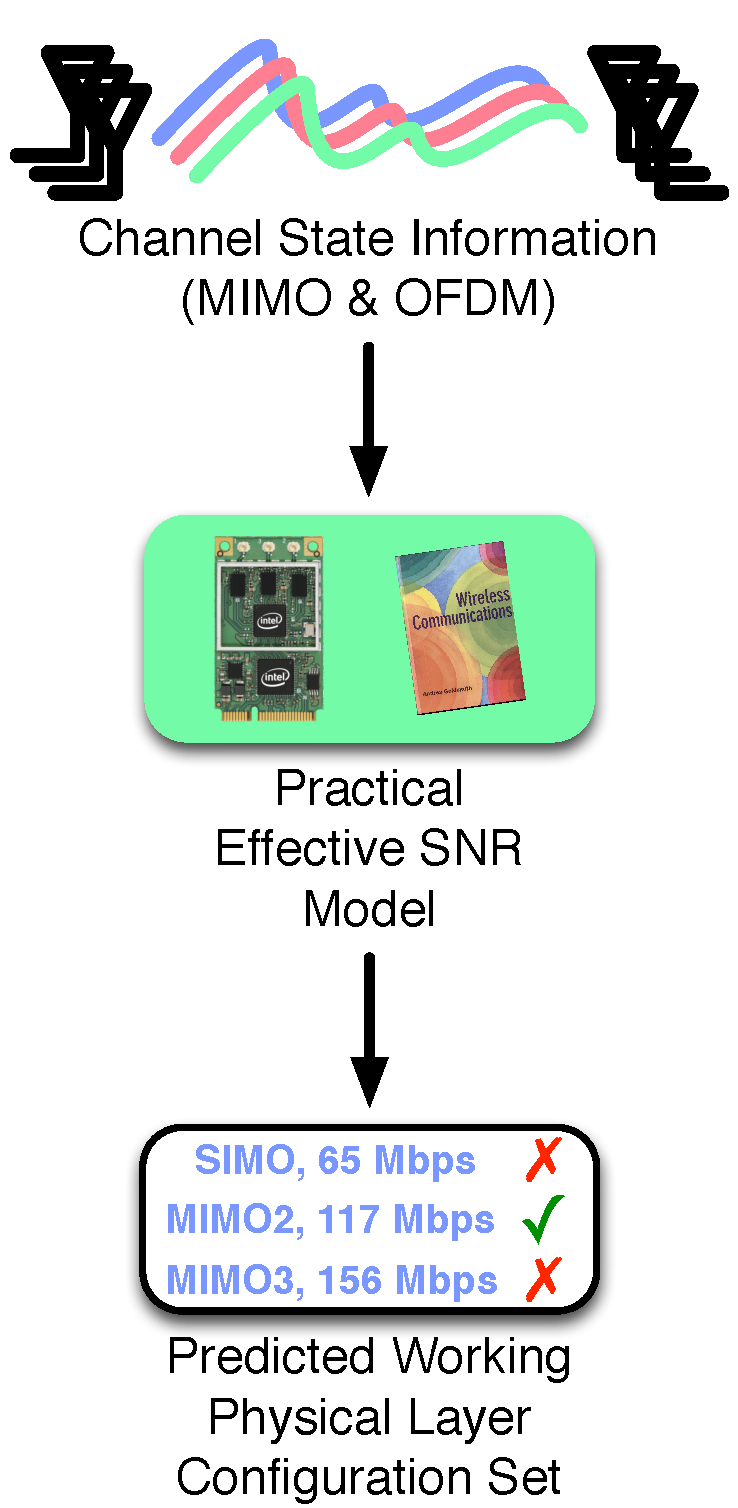
\includegraphics[width=2.2in]{figures/introduction/rate_selection_esnr.pdf}
	\caption[Effective SNR-based approach to making application decisions]{\label{fig:selection_esnr}An Effective SNR-based approach to making application decisions in 802.11n networks.}
\end{figure}

\figref{fig:selection_esnr} presents a pictorial summary of my approach. This approach is closely related to the ``theoretical approach'' presented in \figref{fig:rate_selection_theory}, with a few key differences.

First, a client will measure the \define{channel state information (CSI)} for a wireless link, instead of the RSSI used to compute Packet SNR today. I described above the key problem with RSSI: It simply measures the total amount of power in a link, which does not capture the properties of the different frequency and spatial subchannels that Wi-Fi uses to send independent data. In contrast, the CSI is a fine-grained measurement that can capture details at the levels of frequency-selective fading (to understand performance under OFDM) and independent spatial paths (to understand performance when using MIMO).
%I noted earlier that Packet SNR computed from RSSI has never been used as an accurate predictor of packet delivery for Wi-Fi networks because it does not capture enough information about the wireless channel; I will present experimental data that confirms this result in \chapref{chap:delivery}. In contrast,
My thesis will show that the low-level measurements comprised by the CSI are fine-grained enough to be useful.

The second step uses the main contribution of my thesis: \emph{A practical Effective SNR-based model for wireless packet delivery}. My model uses the measured CSI as input, and incorporates textbook algorithms, ideas from communications theory, as well as some implementation-specific details to handle a wide variety of channels, hardware devices, and applications. At the core of my model is the notion of \define{Effective $E_b/N_0$}, described in a seminal 1998 paper by Nanda and Rege~\cite{Nanda_EffectiveSNR}. The Effective $E_b/N_0$ is defined in the context of links with faded subchannels, either time-varying as in Nanda and Rege's initial work, frequency-selective as with 802.11n OFDM, or spatially-variant with 802.11n MIMO. The Effective $E_b/N_0$ for a faded link is a number, defined as the signal-to-noise ratio that describes the power of a flat link with the same error performance as the link studied. An Effective SNR\footnote{In electrical engineering literature, $E_b$ denotes the energy of a bit and $N_0$ denotes the noise floor, so $E_b/N_0$ is the signal-to-noise ratio of a single bit. In the context of 802.11, in which SNR is derived from RSSI, we use a slightly different definition of SNR that is not normalized by the number of bits.} model aims to compute the Effective SNR using information about the variation of fading across the different subchannels.

The output of the model is a set of Effective SNR values, one for each studied physical-layer configuration. These can then be used to compute a predicted \emph{set of working physical layer configurations}. For each physical layer configuration in the application space---which can span the choice of modulation, coding scheme, transmit or receive antenna set, and more---the model predicts how well that configuration is likely to deliver packets. The application can then choose among the configurations in a way that optimizes its objective function. My thesis includes a detailed description of how my model can be used to solve general classes of wireless network configuration problems, and comprehensive evaluations for the key applications that arise in device-to-device networks.

\section{Hypothesis and Contributions}
I use this approach to demonstrate my hypothesis that \emph{it is possible to rapidly and accurately predict how well different configurations of MIMO and OFDM wireless links will perform in practice, using a small set of wireless channel measurements}.

My Effective SNR-based model takes as input only a single CSI measurement for a wireless link, and from this can compute a predicted Effective SNR value for every point in the configuration space of that link. Predictions can be used for rate selection, because they will indicate the fastest rate to use, but also support concurrent adjustment of factors such as antenna selection, spatial streams, and transmit power level. For multi-device problems such as access point or channel selection, my model requires only a single CSI measurement for each link involved, and thus my model can cover a larger configuration space with only a small set of channel measurements.

The channel state information, like RSSI, is estimated by a receiver using only the preamble of a received packet. This means that unlike packet delivery probes, CSI measurements can be obtained sending only short packets with no payloads. My single-threaded implementation can compute all the Effective SNR values for a 3x3-antenna, 20\MHz 802.11n link in under 4\us, less than a single Wi-Fi packet preamble. The combined process of CSI measurement Effective SNR computation is so fast that predictions of how well links can work can be fed back into control algorithms at near-instantaneous timescales compared to sending a single data-laden packet.
%This shows that the process enables rapid predictions and quick adaptation of link and network configurations.
In addition to quick measurement and decision, there is little information sharing required in order to enable configuration decisions across links. As a result the network can rapidly respond to varying wireless channels.

I emphasize that my model is practical. To demonstrate my hypothesis, I prototype my Effective SNR-based model in the context of 802.11n using commodity Intel Wi-Fi devices. The model is designed to integrate into modern wireless systems, including the practical implementation aspects of real hardware. Using this practical model and prototype, I demonstrate that my model can make accurate predictions of packet delivery. Thus my model provides good performance in practice. My thesis includes an in-depth evaluation of my model in the context of many wireless link and network applications.

%Throughout this thesis, I describe the components of this approach in detail. The organization of this thesis is presented below in \secref{sec:intro_organization}.

%\subsection{Better Physical Layer Measurements}
%The input to my model is a detailed measurement of the physical layer known as the Channel State Information (CSI). Compared to the Packet SNR metric computed from RSSI, which summarizes the total power measured by each antenna, the CSI describes the wireless properties of each of the frequency (OFDM) and spatial (MIMO) subchannels. 
%
%%The 802.11n standard released in 2009 adds a new Channel State Information (CSI)~\cite[\S7.3.1.27]{80211n} measurement facility in order to support multi-antenna (Multiple-Input-Multiple-Output, or MIMO) operation. Devices that report the CSI can provide channel measurements at the level of individual OFDM subcarriers and individual spatial paths. These measurements form a much richer set of information about the RF channel than does the RSSI.
%
%To compare the CSI with Packet SNR, consider an 802.11n link with $M$ antennas at the transmitter and $N$ at the receiver. Today's receivers measure $N$ RSSI values, each corresponding to the total power measured at one receive antenna. In contrast, the CSI contains $M$$\times$N$\times$$S$ values, where $S$ is the number of subcarriers measured. This results in a factor of $MS$ more channel measurements when measuring CSI as opposed to SNR\@. In 802.11, the CSI can measure from 1 to 4 antennas, and from 16 to 114 subcarriers. The CSI thus includes between 16$\times$ and $456\times$ as many measurements as the RSSI\@.
%
%\subsection{A Practical Effective SNR Model}
%The CSI gives fine-grained channel measurements that capture the low-level details of the physical RF channel, but this does not on its own give an accurate predictor of packet delivery. The second step in my approach is to use the detailed information provided by CSI as input to a model of a wireless link. A recent body of theoretical work on measuring and predicting the error performance of wireless channels that are faded, use OFDM, or use MIMO. Chief among these is the seminal 1998 paper by Nanda and Rege on the concept of \define{Effective $E_b/N_0$}~\cite{Nanda_EffectiveSNR}, which forms the theoretical basis of my model for 802.11n MIMO-OFDM channels. 
%
%I give a detailed description of the Effective SNR concept and how I model it in a practical system in a subsequent chapter (\chapref{chap:model}). Briefly, the goal of the Effective SNR is to to give a channel quality metric that reflects the \emph{actual error rate of the link} taking into sub-channel effects like fading. The Effective SNR of a faded channel is defined as the SNR in an equivalent constant-SNR channel that would yield the same error performance. Another way to think about this is that the SNR reports the \emph{total power} received, whereas the Effective SNR reports the amount of \emph{useful power} received. As I will show in this thesis, because Effective SNR accurately reflects packet delivery it can be used to inform a wide variety of configuration decisions about 802.11n systems.

%In my thesis, I take advantage of these three points to build a practical system to return to the ``traditional'' algorithm and predict wireless error performance from channel measurements. Rather than the ``try-it-and-see'' adaptation algorithms in use today, my model enables measurement-based selection of operating points for a wide range of transmitter and receiver parameters over a large application space.

%The opportunity to make progress has arisen for two reasons. First, 802.11n devices measure the channel at the level of individual OFDM subcarriers and individual spatial paths to support 802.11n MIMO (multi-antenna) operation. They report this information in a standard Channel State Information (CSI) format~\cite[\S7.3.1.27]{80211n}. This provides a much richer source of information than SNR\@. Note that this CSI naturally applies to 802.11a/g rates because they are a subset of 802.11n rates. Second, modern NICs use OFDM, which gives channel estimates that are less susceptible to interference than spread spectrum (because of lower correlation), and are calibrated. Both factors lead to more meaningful measurements than in the past.


%\subsubsection{Better Channel Measurements}
%The chief problems with using channel measurements available in commodity Wi-Fi devices is that they only describe the SNR, a measure of total power in the channel. Even if they did not suffer from the hardware artifacts described above, this information would insufficiently describe the wireless channel, because bits are no longer spread across the entire band as in 802.11b modes, but instead are sent independently on different frequencies (called subcarriers) with orthogonal frequency division multiplexing (OFDM), and on different spatial paths with 802.11n multi-antenna techniques.
%
%As part of my thesis, I built a tool (described in \secref{sec:tool}) to measure the channel in a fine-grained manner that accurately reflects the underlying radio channel. In particular, this tool can measure the 802.11n Channel State Information (CSI)~\cite[\S7.3.1.27]{80211n} for each received 802.11n packet. The CSI measures not just the SNR of the entire channel, but instead the channel response at the level of individual subcarriers and spatial paths. For comparison, for an 802.11n link with the antennas each at the transmitter and receiver, today's receivers measure three SNR values each corresponding to the total power measured at a receive antenna. In contrast, the CSI contains 3$\times$3$\times$$S$ values, where $S$ is the number of subcarriers measured. Since 802.11n links use either 56 or 114 subcarriers, $S$ could be as high as 56; in practice, our tool can only measure a subset of 30 of them. Still, this results in 270 channel measurements using the CSI, compared to only 3 with the traditional SNR\@.
%My tool uses a commercially-available Intel Wi-Fi device that supports 802.11n. I modified the open-source Linux drivers, and---in conjunction with Intel Research---the firmware for these devices to enable debug modes with 
%\subsubsection{Effective SNR}


%%%%%%%%%%%%%%%%%%%%%%%%%%%%%%%%%%
\subsection{Contributions}
\label{sec:intro_contributions}

To summarize, the contributions of this thesis are as follows:
\begin{itemize}[leftmargin=0.5cm,parsep=1ex,itemsep=1ex,topsep=1ex]
\item I develop a model that accurately predicts the error performance of different MIMO and OFDM configurations on wireless channels. This model is flexible to support a wide variety of transmitter and receiver device capabilities, device implementations, and applications. I present an implementation of my model using a commodity 802.11n wireless device that demonstrates its feasibility in practice and handles the practical considerations of operation over real links using real, non-ideal hardware. This includes a detailed experimental evaluation of my system that shows that this model accurately predicts packet delivery over real 802.11n wireless links in practice.

\item I detail how to use this model in a system that can solve a large number and variety of configuration problems similar to those described in \secref{sec:intro_problem}. I evaluate this system in the context of a wide variety of 802.11n configuration problems.
%In these evaluation, I quantify the performance gains when using my Effective SNR metric over versions that use the RSSI-based SNR channel measurements available today.
These evaluations show that the predictions output by my model lead to good application performance in practice, and exceed the performance of prior probe-based and RSSI-based approaches.

\item As part of my thesis I have produced an 802.11n research platform based on open-source Linux kernel drivers, open-source application code, and commodity Intel 802.11n devices using closed-source firmware that I customized.
%that uses commodity 802.11n wireless devices to measure the 802.11n CSI for the wireless channel, and use this tool to apply my model to real measured 802.11n channels.
I have released this tool publicly, and at the time of writing it is in use at 23 universities, research labs, and corporations.
\end{itemize}

%%%%%%%%%%%%%%%%%%%%%%%%%%%%%%%%%%
\section{Organization of this Thesis}
\label{sec:intro_organization}
The rest of this thesis is organized as follows. In \chapref{chap:background}, I provide background information on wireless signals and systems in general, and the IEEE 802.11 standards in particular. \chapref{chap:problem} introduces the problem with using channel measurements to predict wireless link performance in today's hardware and using today's techniques, and introduces my Effective SNR-based approach to solving it. In \chapref{chap:model}, I develop my Effective SNR model for 802.11n link performance, and demonstrate its ability to handle a wide range of transmitter and receiver configurations as well as wireless applications. I describe my measurement tool and experimental apparatus in \chapref{chap:tool}. I use this platform to evaluate the ability of my model to predict error performance over a single link in \chapref{chap:delivery}. Next, I conduct a detailed study of the model in the context of rate selection for 802.11n in \chapref{chap:rate}, and then present brief results for a variety of other applications in \chapref{chap:applications}. I place this thesis in the context of related work in \chapref{chap:related}. Finally, I present concluding thoughts along with a brief discussion of the next steps for this work in \chapref{chap:conclusion}.

%%%%%%%%%%%%%%%%%%%%%%%%%%%%%%%%%%
\ifx\mainfile\undefined
%
% ==========   Bibliography   ==========
%
%\nocite{*}   % include everything in the uwthesis.bib file
\bibliographystyle{plain}
\bibliography{dhalperi_thesis}

\end{document}
\fi
